\chapter{Analyse}

\section{Recherche}

\subsubsection{Bezeichnung}
Der Ausdruck \gls{glos:droneLabel} kommt vom niederdeutschen Wort \textit{"`drone"'}, welches wiederum seinen Ursprung beim indogermanischen Wort \textit{"`dhren"'} findet. Die Bedeutung dieses Wortes lautet "`brummen"' oder "`dröhnen"'. \footcite{Geschichte_der_Drohne_-_Nachrichten_Print_-_DIE_WELT_-_Wissen_Print_DW_-_DIE_WELT_2015-03-21}

\begin{framed}
	\textit{Definition: }\textbf{\gls{glos:droneLabel}}\\
	Als \gls{glos:droneLabel} wird ein unbemanntes Luftfahrzeug bezeichnet. Die Steuerung kann entweder manuell oder autonom erfolgen.\\
	Quelle: 
	\cite{Drone_Define_Drone_at_Dictionary.com_2015-03-21}
\end{framed}

\subsection{Geschichte der Drohne}

\subsection{Frühe Entwicklung}
Eine der allerersten bekannten \gls{glos:droneLabel} war wohl von den Brüder Mongolfier (1783) aus Frankreich, ein unbemannter Heissluftballon. \footcite{Kleine_Geschichte_der_Drohnen_-_Nachrichten_Print_-_WELT_KOMPAKT_-_Lifestyle_-_DIE_WELT_2015-03-21}
\footcite{Unbemannte_Luftfahrt__Wikipedia_2015-03-22}

\subsection{Waffenträger}
Später wurde das Potenzial von \glspl{glos:droneLabel} besonders für kriegerische Zwecke erforscht und entwickelt.

\begin{wrapfigure}{r}{0.4\textwidth}
	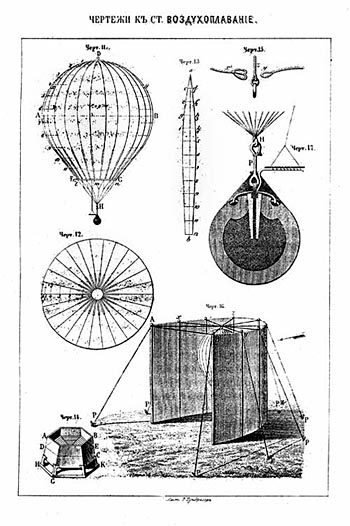
\includegraphics[width=1.0\linewidth]{images/analysis/balloonbombs1849.jpg}
 	\caption[Bombing by Balloon, 1848]{Bombing by Balloon, 1848 \protect\footcite{Remote_Piloted_Aerial_Vehicles_2015-03-21}}
\end{wrapfigure}

So wurden bereits 1849, vom österreichischen Königsreich, unbemannte Heissluftballone mit Bomben im Krieg gegen Venedig losgeschickt.
Weder die "`\gls{glos:droneLabel}"' selbst, noch das Abwerfen der Bombe konnte aktiv gesteuert werden.
Die Heissluftballone flogen mit dem Wind und die Bomben wurde per Zeitzünder gezündet. Tatsächlich erreichten einzelne Ballone ihr Ziel und konnten Schaden anrichten, andere jedoch wurden vom Wind zurück geweht und zerstörten das eigene Territorium Österreichs. \footcite{Remote_Piloted_Aerial_Vehicles_2015-03-21}

Während dem \textit{Ersten Weltkrieg} wurden die ersten unbemannten Flugzeuge von den Amerikanern entwickelt.
Mit diesen wurden vordefinierte Routen abgeflogen und es konnten \textit{Flugtorpedos} abgeworfen werden, welche wie die Flugzeuge selbst, mit Hilfe von gyroskopischen Stabilisierer und Aneroidbarometer zwar Richtung und Höhe halten konnten, jedoch nicht per Funk steuerbar waren.

Die ersten funkgesteuerten \glspl{glos:droneLabel} wurde erst nach dem Krieg 1918 fertig.
Nebst den Amerikanern, hatten auch die Briten 1925 ihren ersten Drohnenflug durchgeführt. Diese konnte etwa 300\,Meilen (ca. 483\,km) mit einer Geschwindigkeit von 190\,mph (ca. 306\,km/h) zurücklegen.\footcite{Informatik_und_Gesellschaft_2015-03-21}

Da der Krieg vorbei war, wurden die \glspl{glos:droneLabel} hauptsächlich für Jagd-Trainings der Armee genutzt.

Mit den Jahren wurden die \glspl{glos:droneLabel} immer weiter verbessert und werden heute aktiv gegen terroristische Aktivitäten verwendet.

\subsection{Weitere Zwecke}
% http://diepresse.com/home/politik/innenpolitik/1385181/Die-Geschichte-der-Drohnen
Nebst den erwähnten Waffenträger gibt es auch diverse weitere Aufgaben für \glspl{glos:droneLabel}: Beobachtungen (z.B. Aufklärungen, Luftaufnahmen, Wetterbeobachtungen, Filmproduktionen), Messungen an Orten die für Menschen ungeeignet oder schädlich sind oder Transporte.

Obschon viele Aufgabenbereiche gewaltfrei sind, dienen \glspl{glos:droneLabel} trotzdem mehrheitlich polizeilichen oder militärischen Organisationen.\footcite{Die_Geschichte_der_Drohnen_DiePresse.com_2015-03-21}

\subsection{Heutige Einsätze von Drohnen}
Seit 2013 werden, in Grand Forks County im US-Bundesstaat North Dakota, \glspl{glos:droneLabel} zur Verbrecherjagd eingesetzt, resp. zur Personensuche.

Auch Amazon kündet ihren "`\textit{Prime Air}"'-Service an, der Pakete direkt vor die Haustür liefert.

Im Jahr 2014 wurde der Einsatz für landwirtschaftliche Zwecke erprobt und auch die \gls{glos:dhlLabel} führte Testlieferungen mit \glspl{glos:droneLabel} aus. \footcite{Kleine_Geschichte_der_Drohnen_-_Nachrichten_Print_-_WELT_KOMPAKT_-_Lifestyle_-_DIE_WELT_2015-03-21}


\section{Quadrocopter}
\begin{wrapfigure}{r}{0.4\textwidth}
	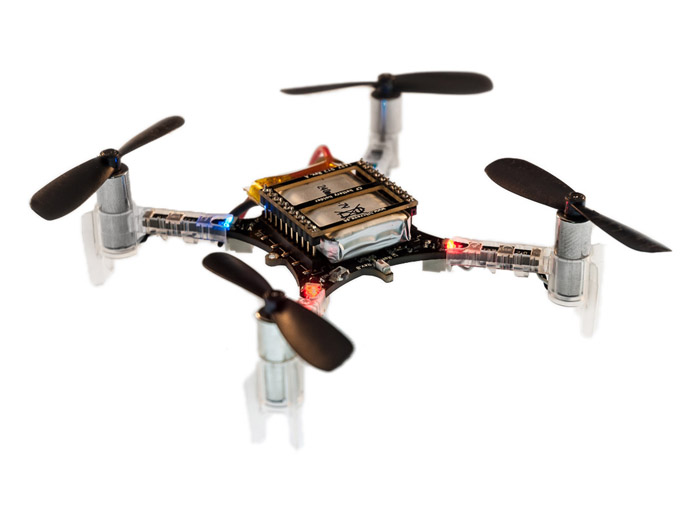
\includegraphics[width=1.0\linewidth]{images/analysis/crazyflize.jpg}
	\caption[Crazyflie 2.0]{Crazyflie 2.0 \protect\footcite{Crazyflie_2.0_Seeedstudio_2015-03-22}}
\end{wrapfigure}
Der Quadrocopter eignet sich als \gls{glos:droneLabel}, da die Steuerung ausschliesslich über die vier Rotoren realisiert wird.
Weitere mechanische Steuerkomponente entfallen, was die Komplexität des Luftfahrzeuges deutlich vereinfacht.
Je zwei der Rotoren drehen in dieselbe Richtung (im bzw. gegen den Uhrzeigersinn) und stehen sich gegenüber.

\subsection{Steuerung}
Bezüglich der Flugeigenschaften entspricht ein Quadrocopter am ehesten einem Hubschrauber und gehört ebenfalls zur Kategorie der  \gls{glos:vtolLabel}-Flugzeugen.
Es sind jegliche Steuermöglichkeiten im dreidimensionalen Raum möglich (steigen/sinken "`\textit{thrust}"', gieren/drehen "`\textit{yaw}"', nicken "`\textit{pitch}"' und rollen "`\textit{roll}"').

Durch das, dass die Rotoren in entgegengesetzte Richtungen drehen, hebt sich das auf das Traggestell übertragene Drehmoment auf und der Quadrocopter kann ohne Drehung fliegen.
Um sich nun in eine Richtung zu \textit{gieren}, werden die Drehzahlen von jeweils zwei gegenüberliegende Rotoren gleichmässig verändert, so dass der Drehmoment auf das Traggestell nicht mehr neutralisiert wird und sich so eine Drehung ergibt.

Um dem Piloten die Steuerung zu erleichtern, befinden sich oft verschiedenfarbige Markierungen oder LED's an der Vorder- oder Rückseite des Quadrocopters.
Die Steuerung erfolgt üblicherweise aus relativer Sicht der Drohne und erfordert somit ein Umdenken des Piloten.\footcite{Quadrocopter__Wikipedia_2015-03-22}


\subsection{Bereits bestehende Arbeiten}

\subsubsection{Steuermöglichkeiten}

\subsubsection{Sensoren Integration auf bestehende Steuerungen}

%%% 
%todo correct
\section{Ist-Analyse}

\begin{wrapfigure}{r}{0.4\textwidth}
	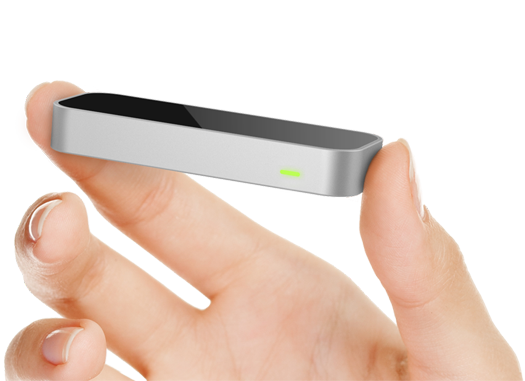
\includegraphics[width=1.0\linewidth]{images/analysis/leap_simple.png}
	\caption[Leap Motion Sensor]{Leap Motion Sensor\protect\footcite{Move_Over_Kinect:_Early_Gestural_Musical_Demos_for_Leap_Motion_Look_Terrific_-_Create_Digital_Music_2015-03-27}}
\end{wrapfigure}
\subsection{Gestensensor} \label{subsec:leapmotion}
%\begin{wrapfigure}{l}{0.4\textwidth}
%	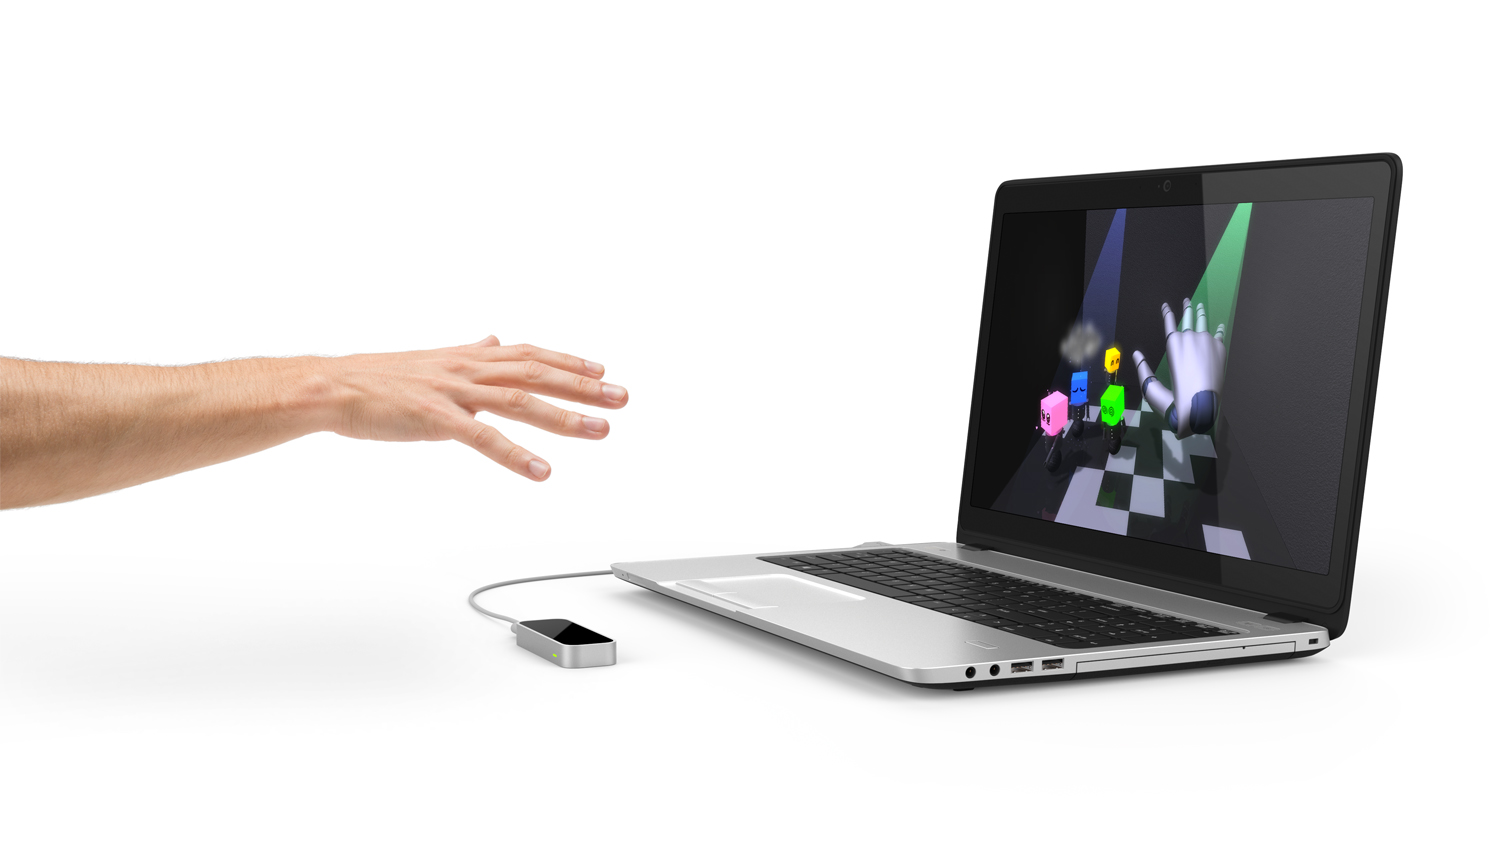
\includegraphics[width=1.0\linewidth]{images/analysis/leap_laptop.jpg}
%	\caption[Leap Motion -- Produktbild]{Leap Motion -- Produktbild \protect\footcite{Leap_Motion_Motion_Controller_2015-03-27}}
%\end{wrapfigure}

Für die Erkennung der Gesten wird der \textit{Leap Moption}\footcite{Leap_Motion_Motion_Controller_2015-03-27} Sensor verwendet.
Dieser erkennt Hände (inkl. einzelne Finger) und stellt Daten deren Position, Gesten und Bewegungen zur Verfügung.

\subsubsection{Technische Details}
Die Erkennung erfolgt via optische Sensoren und Infrarot Licht.
Der Leap Motion wird per USB 2.0 angeschlossen und erkennt Gesten innerhalb eines 150\textdegree-Winkels zwischen 25\,mm und 600\,mm Höhe.
Am besten funktioniert der Sensor, wenn die Silhouette der Hand mit hohem Kontrast zur Umgebung unterschieden werden kann.
Die Messdaten werden mit einem internen Handmodell kombiniert, um so immer eine vollständige Hand erkannt zu haben.
\footcite{API_Overview__Leap_Motion_v2.2_documentation_2015-03-27}


\begin{figure}[H]
  \IfDefined{RawFloats}{\RawFloats} % required if floatrow is loaded
  \begin{minipage}[b]{0.45\linewidth}
    \centering
   	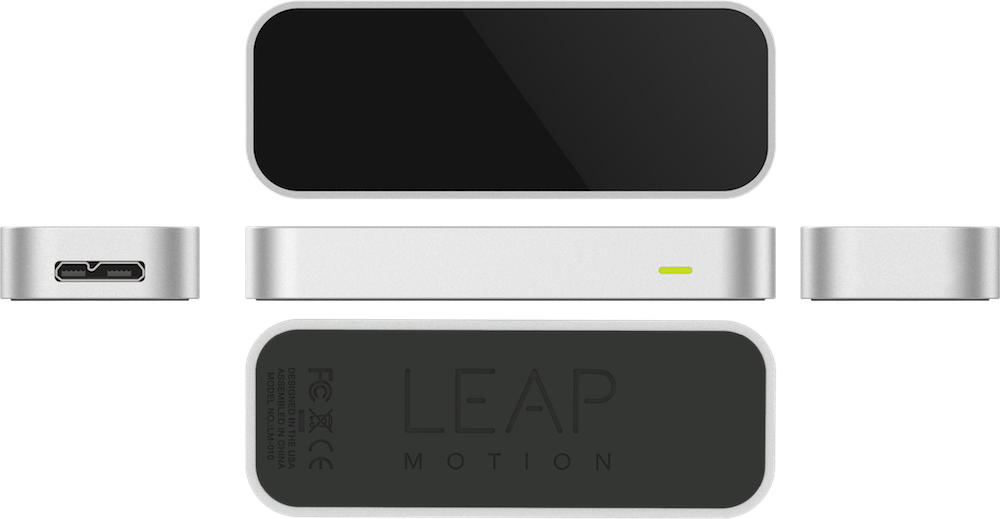
\includegraphics[width=1.0\linewidth]{images/analysis/leap_360_view.png}
   	\caption[Leap Motion von allen Seiten]{Leap Motion von allen Seiten \protect\footcite{Leap_Motion_-_VJs_Magazine_2015-03-27}}
  \end{minipage}%
  \hspace{.1\linewidth}
  \begin{minipage}[b]{0.45\linewidth}
    \centering
	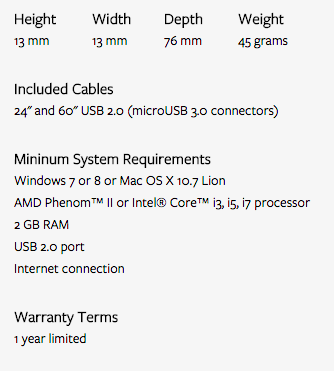
\includegraphics[width=1.0\linewidth]{images/analysis/leap_technical_specifiaction.png}
	\caption[Leap Motion -- Technische Spezifikationen]{Leap Motion -- Technische Spezifikationen \protect\footcite{Leap_Motion_Motion_Controller_2015-03-27}}
  \end{minipage}
\end{figure}

Weitere Informationen könne übersichtlich auf der Website des Herstellers\footcite{Leap_Motion_Motion_Controller_2015-03-27} gefunden werden.


\begin{wrapfigure}{r}{0.4\textwidth}
	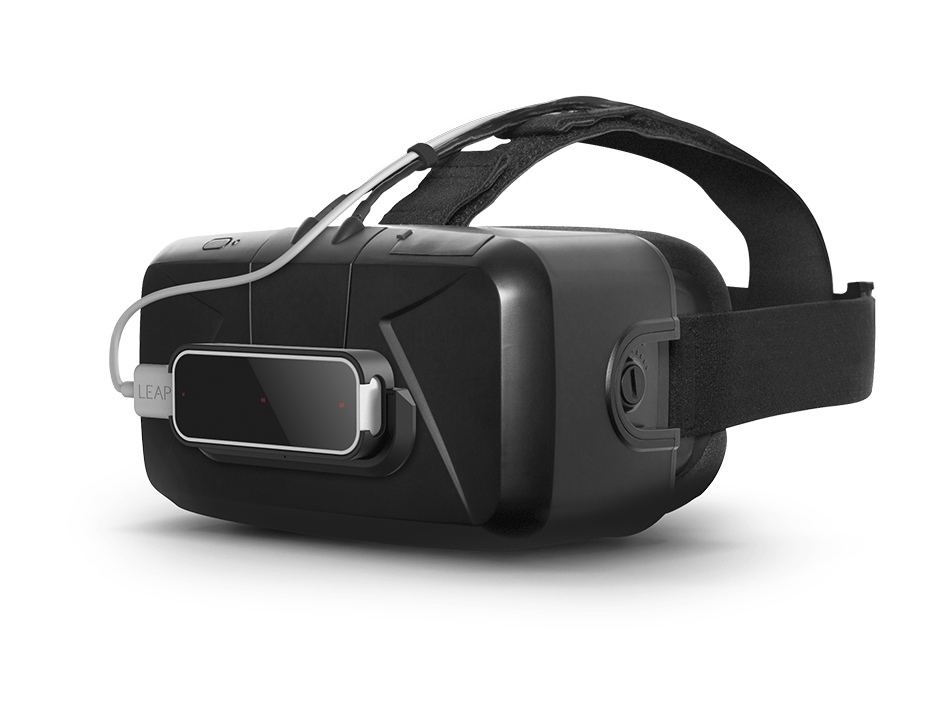
\includegraphics[width=1.0\linewidth]{images/analysis/leap_vr.png}
	\caption[Oculus Rift VR]{\gls{vrLabel} Oculus Rift \protect\footcite{Leap_Motion_Developers_2015-03-27}}
\end{wrapfigure}
\subsubsection{Anwendungsbereich}
Der Anwendungsbereich für Gestenerkennung ist beinahe grenzenlos.
Da der Leap Motion speziell für Entwickler produziert wurde, kann der Sensor für jegliche Programme oder Steuerungen verwendet werden.

Gestensteuerungen sind für "`gewöhnliche"' Steueraufgaben nach wie vor sehr wenig verbreitet, obwohl es theoretisch nichts intuitiveres als Gesten gibt.
Dies kann unter anderem an fehlenden Anwendungsfällen oder an falsch angesetzten Umsetzungen liegen.



\subsubsection{Einrichtung}



\subsubsection{API}
% sprachen
% Aufbau der Antworten




\subsection{Drohne}

\subsubsection{API}

\subsubsection{Sensoren charakterisieren}


%%% 

\section{Soll-Analyse}
\subsection{Gesten-Steuerbeschrieb}


%%% 
